%%%%%%%%%%%%%%%%%%%%%%%%%%%%%%%%%%%%%%%%%
% fphw Assignment
% LaTeX Template
% Version 1.0 (27/04/2019)
%
% This template originates from:
% https://www.LaTeXTemplates.com
%
% Authors:
% Class by Felipe Portales-Oliva (f.portales.oliva@gmail.com) with template 
% content and modifications by Vel (vel@LaTeXTemplates.com)
%
% Template (this file) License:
% CC BY-NC-SA 3.0 (http://creativecommons.org/licenses/by-nc-sa/3.0/)
%
%%%%%%%%%%%%%%%%%%%%%%%%%%%%%%%%%%%%%%%%%

%----------------------------------------------------------------------------------------
%	PACKAGES AND OTHER DOCUMENT CONFIGURATIONS
%----------------------------------------------------------------------------------------

\documentclass[
	french,
	11pt, % Default font size, values between 10pt-12pt are allowed
	%letterpaper, % Uncomment for US letter paper size
	%spanish, % Uncomment for Spanish
]{fphw}

% Template-specific packages
\usepackage{babel}
\usepackage[utf8]{inputenc} % Required for inputting international characters
\usepackage[T1]{fontenc} % Output font encoding for international characters
\usepackage{mathpazo} % Use the Palatino font
% \usepackage{iwona} % Use the Iwona font

\usepackage{amsmath}
\usepackage{mathtools}

\usepackage{graphicx} % Required for including images
\usepackage[textfont=it]{caption}  %% To manage long captions in images
\usepackage{subcaption}
\captionsetup{justification=centering}

\usepackage{float}
\graphicspath{ {./img/} }

\usepackage{booktabs} % Required for better horizontal rules in tables

\usepackage{listings} % Required for insertion of code

\usepackage{array} % Required for spacing in tabular environment

\usepackage{enumerate} % To modify the enumerate environment

\usepackage{amssymb}
\usepackage{enumitem}	%% % To modify the itemize bullet character
\usepackage{xfrac}

\usepackage{xcolor}
\usepackage{listings}
\colorlet{mygray}{black!30}
\colorlet{mygreen}{green!60!blue}
\colorlet{mymauve}{red!60!blue}
\lstset{
  backgroundcolor=\color{gray!10},  
  basicstyle=\scriptsize\ttfamily,
  columns=fullflexible,
  breakatwhitespace=false,      
  breaklines=true,                
  captionpos=b,                    
  commentstyle=\color{mygreen}, 
  extendedchars=true,              
  frame=single,                   
  keepspaces=true,             
  keywordstyle=\color{blue},      
  language=c++,                 
  numbers=none,                
  numbersep=5pt,                   
  numberstyle=\tiny\color{blue}, 
  rulecolor=\color{mygray},        
  showspaces=false,               
  showtabs=false,                 
  stepnumber=5,                  
  stringstyle=\color{mymauve},    
  tabsize=3,                      
  title=\lstname                
}


\usepackage[linkcolor=blue,colorlinks=true]{hyperref}
\usepackage{cleveref}
\usepackage{siunitx}
\newcommand{\bvec}[1]{\bm{#1}}    %% For vector notation
\newcommand{\myvec}[2]{\begin{pmatrix} #1  \\ #2 \end{pmatrix}}   %% vecteur 2d
\newcommand{\mymat}[4]{\begin{pmatrix} #1 & #2 \\ #3 & #4 \end{pmatrix}}  %% Matrice 2*2
\newcommand{\tabhead}[1]{{\bfseries#1}}
\newcommand{\hquad}{\hspace{0.5em}} %% Bew command for half quad
% \setlength\parindent{0pt}	%% To remove all indentations

\setlength\parindent{0pt}

%----------------------------------------------------------------------------------------
%	ASSIGNMENT INFORMATION
%----------------------------------------------------------------------------------------

\title{TP \#2} % Assignment title

\author{Roussel Desmond Nzoyem} % Student name

\date{\today} % Due date

\institute{Université de Strasbourg \\ UFR de Mathématiques et Informatique} % Institute or school name

\class{EDP 2} % Course or class name

\professor{Pr. Philippe Helluy} % Professor or teacher in charge of the assignment

%----------------------------------------------------------------------------------------

\begin{document}

\maketitle % Output the assignment title, created automatically using the information in the custom commands above

%----------------------------------------------------------------------------------------
%	ASSIGNMENT CONTENT - SECTION 1
%----------------------------------------------------------------------------------------


\section*{Résolution numérique de l'équation de Saint-Venant}

\subsection*{Question 1.}
\begin{problem}
	Calcul numérique au moyen du solveur de Riemann exact fourni, de la solution du problème de Riemann pour le modèle de Saint-Venant.
	\begin{align*}
		\partial_t w + \partial_x f(w) &=0 \\
		w = (h,hu)\\
		f(w) = (hu, hu^2 + gh^2/2) \quad &, \quad g=9.81 \text{ m/s}^2 \tag{1}\\
		u(x,0) &= 0 \\
		h(x,0) &= 
		\begin{cases}
			h_L = 2 \quad \text{si } x<0 \\
			h_R = 1 \quad \text{si } x>0
		\end{cases}
		\label{eq:stVenant}
	\end{align*}
\end{problem}


\subsection*{Réponse} 

Avec le solveur de Riemann en langage C fourni, la fonction de calcul de la solution exacte en découle facilement \footnote{Les conditions initiales qui y sont définies seront les mêmes durant la première partie de ce rapport, et tout changement de ces conditions sera alors explicitement indiqué.}.

\begin{lstlisting}[language=C, caption={Fonction de calcul de la solution exacte},breaklines]
void solexacte(double x, double t, double* w) {
    /* Conditions intiale */
    double hL=2;
    double uL=0;

    double hR=1;
    double uR=0;

	// Variables conservatives
    double wL[2]={hL, hL * uL};		    
    double wR[2]={hR, hR * uR};

	// Calcul du point d'évaluation (variable autosimilaire)
	double z = x/ (t + 1e-12);          
	
	// Solveur de Riemann fourni
    riem_stvenant(wL, wR, z, w);
}
\end{lstlisting}
Le solveur de Riemann exact fourni produit le résultat obtenu à la \cref{fig:SolExacte500} qui nous permet d'observer de façon distincte deux ondes qui se propagent depuis l'origine. Vers la gauche, on a une onde de détente (ou de raréfaction) ($h_L > h^\ast$); et vers la droite, on a une onde de choc ($h^\ast > h_R$). Ici, $h^\ast$ désigne la hauteur d'eau de la zone intermédiaire entre la gauche et la droite au fur et à mesure que les ondes se séparent.
\begin{figure}[h]
	\centering
	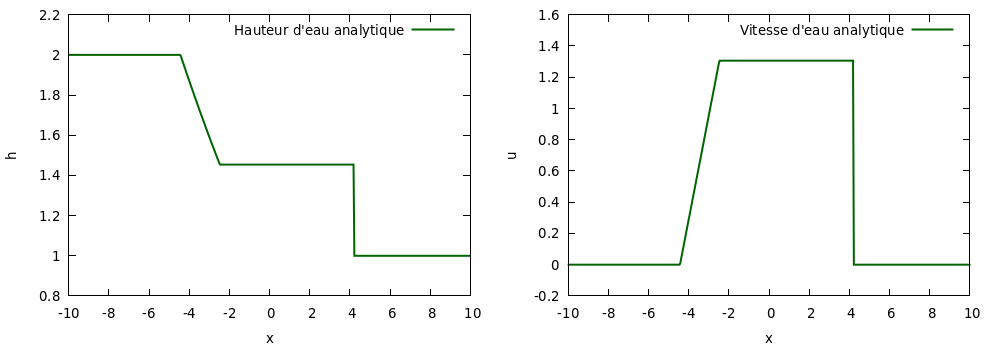
\includegraphics[width=0.8\textwidth]{SolExacte500.png}
	\caption{Solution analytique obtenue à l'aide du solveur de Riemann fourni. A gauche la hauteur d'eau et à droite la vitesse d'eau. $x_{min}=-10$, $x_{max}=10$, $t_{final} = 1$ et le nombre de mailles est de $N=500$.}
	\label{fig:SolExacte500}
\end{figure}


\subsection*{Question 2.}
\begin{problem}
	Programmation du schéma de Godunov et vérification au moyen du cas test indiqué.
\end{problem}


\subsection*{Réponse} 

Le schéma de Godunov consiste appliquer le flux physique à la solution du problème de Riemann à l'interface de deux mailles. 

\begin{lstlisting}[language=C, caption={Programmation du flux numérique de Godunov},breaklines]
void fluxnum(double* a, double* b, double* flux) {
	riem_stvenant(a, b, 0., w);		// solveur fourni
	fluxphy(w, flux);
}
\end{lstlisting}
Un autre élément important dans cette implémentation est la fonction principale de calcul $\verb|godunov_solve|$ \footnote{Les autres fonctions nécessaires découlent immédiatement de la définition du problème, elles ne seront pas détaillées ici.}.

\begin{lstlisting}[language=C, caption={Fonction de résolution du problème de Saint-Venant utilisée dans ce rapport (sauf indication contraire).},breaklines]
void godunov_solve(godunov* gd, double tmax) {
	double tnow = 0;
	int m = gd->m;
	while (tnow < tmax) {
		double vmax = 0;
		// calcul de la vitesse max
		for (int i = 0; i < gd->N + 2; i++) {
			double vloc = lambda_max(gd->un + m * i);
			vmax = vmax > vloc ? vmax : vloc;
		}
		// Pas de temps
		gd->dt = gd->cfl * gd->dx / vmax;
		// Application du flux numerique
		for (int i = 1; i < gd->N + 1; i++) {
			double flux[m];
			double uL[2], uR[2];
			// Application du flux à droite
			fluxnum(gd->un + i * m, gd->un + (i + 1) * m, flux);
			for (int iv = 0; iv < m; iv++) {
				gd->unp1[i * m + iv] =
					gd->un[i * m + iv] - gd->dt / gd->dx * flux[iv];
			}
			// Application du flux à gauche
			fluxnum(gd->un + (i - 1) * m, gd->un + i * m, flux);
			for (int iv = 0; iv < m; iv++) {
				gd->unp1[i * m + iv] += gd->dt / gd->dx * flux[iv];
			}
		}
		// Mise à jour
		tnow += gd->dt;
		// Conditions au bord
		int i = 0;
		solexacte(gd->xi[i], tnow, gd->unp1 + i * m);
		i = gd->N + 1;
		solexacte(gd->xi[i], tnow, gd->unp1 + i * m);
		// Preparation pour la prochaine etape
		memcpy(gd->un, gd->unp1, (gd->N + 2) * m * sizeof(double));
	}
	gd->tfin = tnow;
}	
\end{lstlisting}
Cette implémentation produit le résultat obtenu à la \cref{fig:SolGodunov500} qui permet de confirmer que la programmation de la méthode de Godunov est correcte.
\begin{figure}[h]
	\centering
	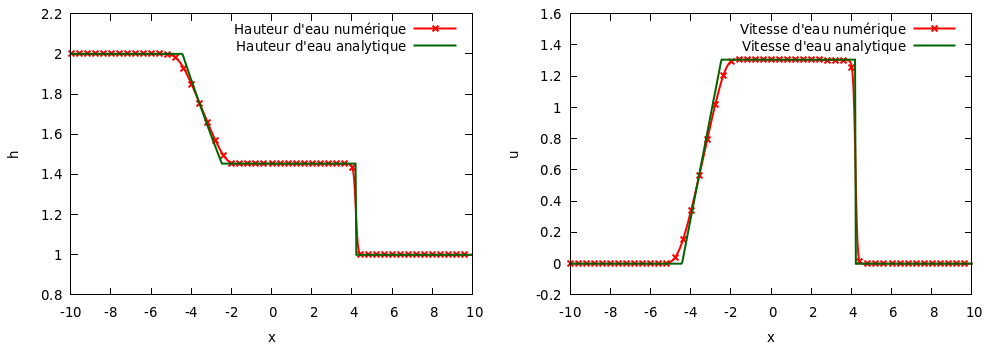
\includegraphics[width=0.8\textwidth]{SolGodunov500.png}
	\caption{Solution numérique obtenue par le schéma de Godunov. $x_{min}=-10$, $x_{max}=10$, $t_{final} = 1$, $CFL=0.5$ et le nombre de mailles est de $N=500$.}
	\label{fig:SolGodunov500}
\end{figure}



\subsection*{Question 3.}
\begin{problem}
	On considère un bassin $[- 10, 10]$ fermé. Le bassin est séparé en deux parties égales grâce à une paroi située en $x = 0$. À l'instant $t = 0$, la partie gauche (respt. droite) est remplie avec de l'eau immobile à une hauteur $h_L$ (respt. $h_R$). À l'instant $t = 0$, on retire la paroi. 
	\begin{itemize}
		\item Écriture et justification de la condition aux limites à imposer en $x = -10$ et $x = 10$.
		\item Nature de cette condition si le bassin est infini.
	\end{itemize} 
\end{problem}


\subsection*{Réponse} 

Pour un bassin fermé, la condition indiquée s'impose par l'application, sur chaque bord, d'une quantité d'eau fantôme, ayant une vitesse opposée à celle des cellules aux bords ($i=0$ ou $i=N+1$)\footnote{L'indice pour la discrétisation en espace est noté $i$, et celui pour la discrétisation en temps $n$.}. Ainsi, à chaque itération $n$, on aura 
\begin{align*}
	h_0^n = h_1^n, &\qquad u_0^n = - u_1^n \\
	h_{N+1}^n = h_N^n, &\qquad u_{N+1}^n = - u_N^n
\end{align*}
En termes de variables conservatives $w=\myvec{h}{hu}$, cela reviens à appliquer 
\begin{align*}
	w_0^n[0] = w_1^n[0], &\qquad w_0^n[1] = - w_1^n[1] \\
	w_{N+1}^n[0] = w_{N}^n[0], &\qquad w_{N+1}^n[1] = - w_{N}^n[1]
\end{align*}
Cette condition traduit le retour de la colonne d'eau après son rebond sur le bord du bassin.

\begin{lstlisting}[language=C, caption={Implementation des conditions aux limites pour un bassin fermé.},breaklines]
	int i = 0;
	gd->unp1[i*m] = gd->unp1[(i+1)*m];
	gd->unp1[i*m+1] = -gd->unp1[(i+1)*m+1];
	i = gd->N + 1;
	gd->unp1[i*m] = gd->unp1[(i-1)*m];
	gd->unp1[i*m+1] = -gd->unp1[(i-1)*m+1];
\end{lstlisting}

En ce qui concerne une piscine infinie, la vague fantôme opposée à l'écoulement est remplacée par une vague dans le même sens que le flux d'eau. Numériquement, cela se traduit par
\begin{align*}
	h_0^n = h_1^n, &\qquad u_0^n = u_1^n \\
	h_{N+1}^n = h_N^n, &\qquad u_{N+1}^n = u_N^n
\end{align*}
\begin{lstlisting}[language=C, caption={Implementation des conditions aux limites pour un bassin infini.},breaklines]
	int i = 0;
	gd->unp1[i*m] = gd->unp1[(i+1)*m];
	gd->unp1[i*m+1] = gd->unp1[(i+1)*m+1];
	i = gd->N + 1;
	gd->unp1[i*m] = gd->unp1[(i-1)*m];
	gd->unp1[i*m+1] = gd->unp1[(i-1)*m+1];
\end{lstlisting}


\subsection*{Question 4.}
\begin{problem}
	\begin{itemize}
		\item Calcul de l'évolution de la surface d'eau au cours du temps. Représentation de $h$ et $u$ à divers instants pour diverses finesses de maillage.
		\item Comparaison avec la solution exacte du problème de Riemann (solution analytique).
	\end{itemize}
	 
\end{problem}

\subsection*{Réponse} 

\begin{figure}[H]
	\centering
	\begin{subfigure}[b]{0.9\textwidth}
		\centering
		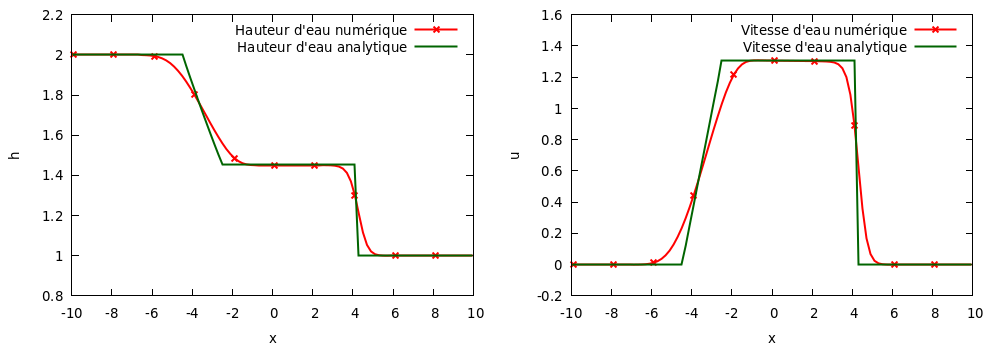
\includegraphics[width=\textwidth]{PiscineBornee1.png}
		\caption{$t_{f}=1$}
		\label{fig:Piscine1A}
	\end{subfigure}
	\begin{subfigure}[b]{0.9\textwidth}
		\centering
		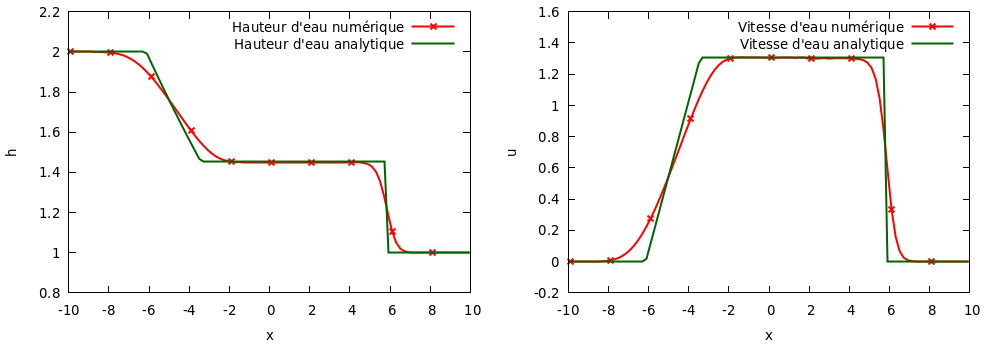
\includegraphics[width=\textwidth]{PiscineBornee2.png}
		\caption{$t_{f}=1.366671$}
		\label{fig:Piscine1B}
	\end{subfigure}
	\begin{subfigure}[b]{0.9\textwidth}
		\centering
		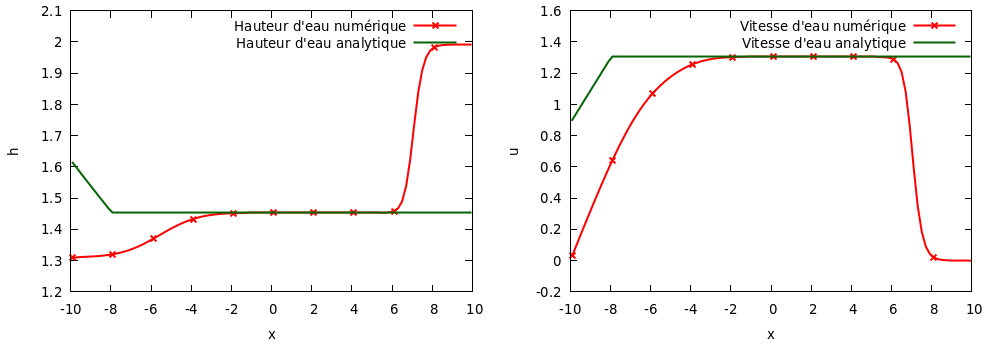
\includegraphics[width=\textwidth]{PiscineBornee3.png}
		\caption{$t_{f}=3.2$}
		\label{fig:Piscine1C}
	\end{subfigure}
	\caption{Évolution de la surface d'eau au cours du temps dans le bassin pour un nombre de mailles $N=100$. Le coefficient $CFL$ vaut $0.5$. La figure (a) montre le système avant d'atteindre les bords, (b) au moment d'arrivée, et (c) après.}
	\label{fig:Piscine1}
\end{figure}

\begin{figure}[H]
	\centering
	\begin{subfigure}[b]{0.9\textwidth}
		\centering
		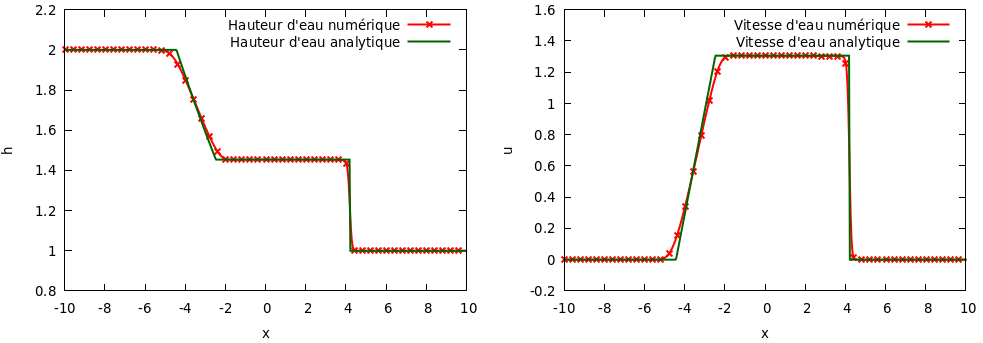
\includegraphics[width=\textwidth]{PiscineBornee4.png}
		\caption{$t_{f}=1$}
		\label{fig:Piscine2A}
	\end{subfigure}
	\begin{subfigure}[b]{0.9\textwidth}
		\centering
		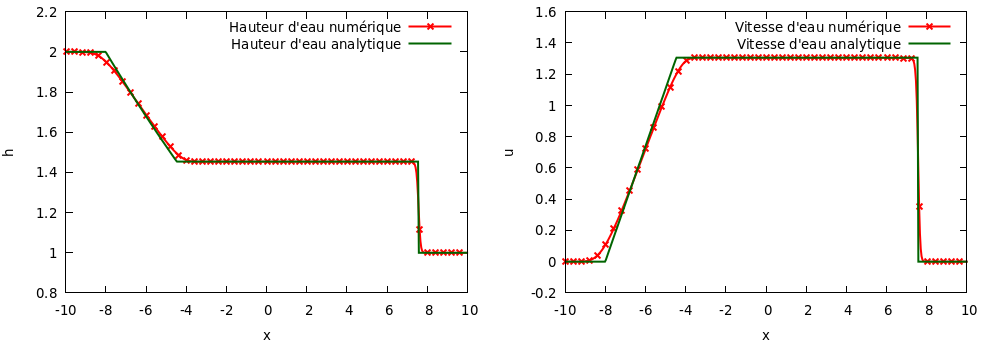
\includegraphics[width=\textwidth]{PiscineBornee5.png}
		\caption{$t_{f}=1.808131$}
		\label{fig:Piscine2B}
	\end{subfigure}
	\begin{subfigure}[b]{0.9\textwidth}
		\centering
		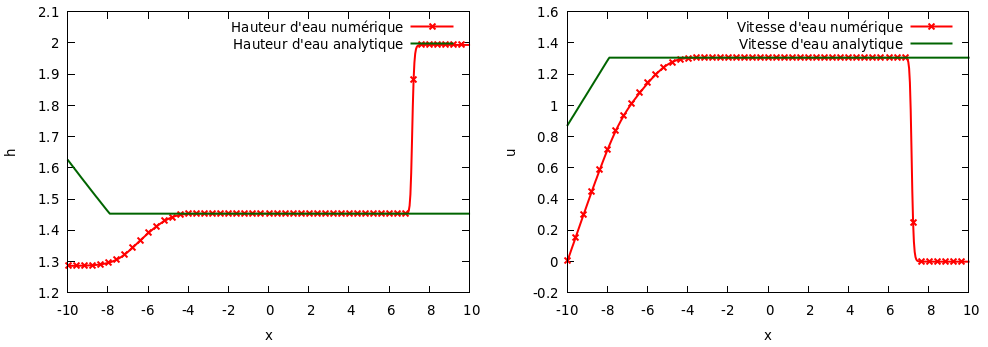
\includegraphics[width=\textwidth]{PiscineBornee6.png}
		\caption{$t_{f}=3.2$}
		\label{fig:Piscine2C}
	\end{subfigure}
	\caption{Évolution de la surface d'eau au cours du temps dans le bassin pour un nombre de mailles $N=500$. Le coefficient $CFL$ vaut $0.5$. La figure (a) montre le système avant d'atteindre les bords, (b) au moment d'arrivée, et (c) après.}
	\label{fig:Piscine2}
\end{figure}

\begin{figure}[H]
	\centering
	\begin{subfigure}[b]{0.9\textwidth}
		\centering
		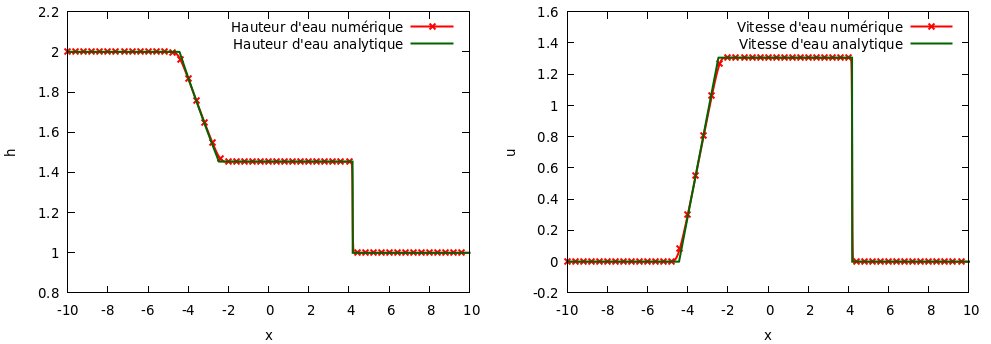
\includegraphics[width=\textwidth]{PiscineBornee7.png}
		\caption{$t_{f}=1$}
		\label{fig:Piscine3A}
	\end{subfigure}
	\begin{subfigure}[b]{0.9\textwidth}
		\centering
		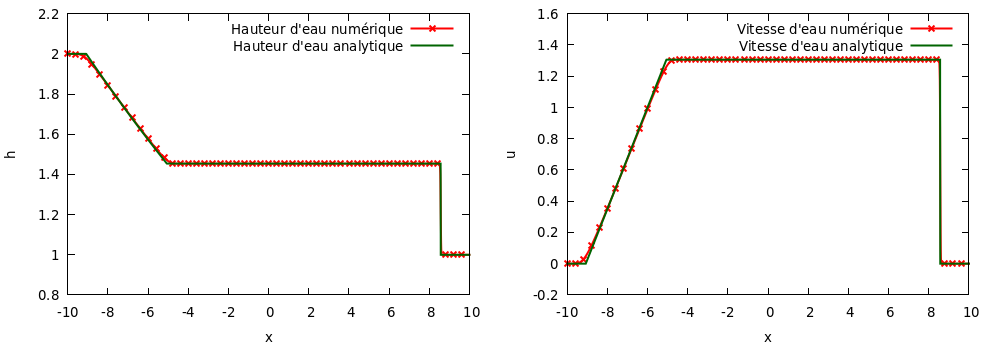
\includegraphics[width=\textwidth]{PiscineBornee8.png}
		\caption{$t_{f}=2.048256$}
		\label{fig:Piscine3B}
	\end{subfigure}
	\begin{subfigure}[b]{0.9\textwidth}
		\centering
		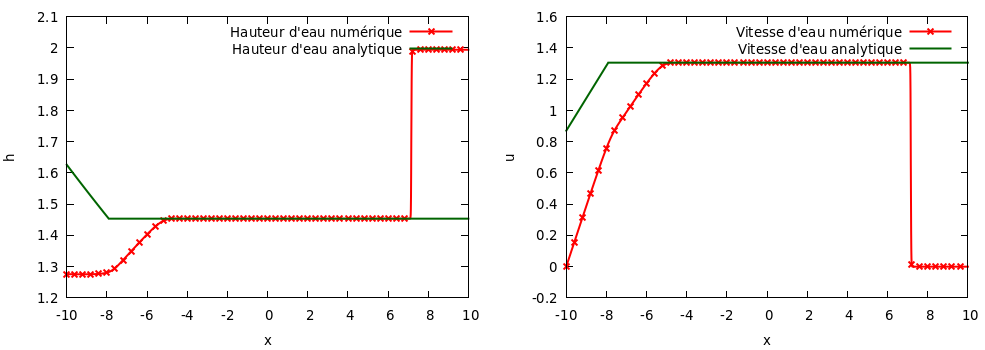
\includegraphics[width=\textwidth]{PiscineBornee9.png}
		\caption{$t_{f}=3.2$}
		\label{fig:Piscine3C}
	\end{subfigure}
	\caption{Évolution de la surface d'eau au cours du temps dans le bassin pour un nombre de mailles $N=2500$. Le coefficient $CFL$ vaut $0.5$. La figure (a) montre le système avant d'atteindre les bords, (b) au moment d'arrivée, et (c) après.}
	\label{fig:Piscine3}
\end{figure}


\noindent Les \cref{fig:Piscine1,fig:Piscine2,fig:Piscine3} illustrent le retour de la colonne d'eau après son rebond sur les bords d'un bassin. Les figures (a) de chaque groupe de figures montrent le système avant d'atteindre les bords. Les figures (b) montrent le moment d'arrivée de la solution numérique, qui marque le début de la différence avec la solution exacte\footnote{À partir des temps indiqués aux figures (b), les solutions analytiques ne sont plus valides.}. Il est intéressant de remarquer que ce temps d'arrivée devient plus précis avec le raffinement du maillage 
\begin{itemize}
	\item $t_{f}=1.366671$ pour $N=100$ (cf. \cref{fig:Piscine1B})
	\item $t_{f}=1.808131$ pour $N=500$ (cf. \cref{fig:Piscine2B})
	\item $t_{f}=2.048256$ pour $N=2500$ (cf. \cref{fig:Piscine3B})
\end{itemize}
Les figures (c) indiquent ce qui se passe après le rebond de la colonne d'eau. On remarque que la solution exacte (solution exacte du problème de Riemann) n'est plus valide après ce rebond, ce qui explique pourquoi les deux solutions diffèrent si largement.


\begin{figure}[H]
	\centering
	\begin{subfigure}[b]{0.9\textwidth}
		\centering
		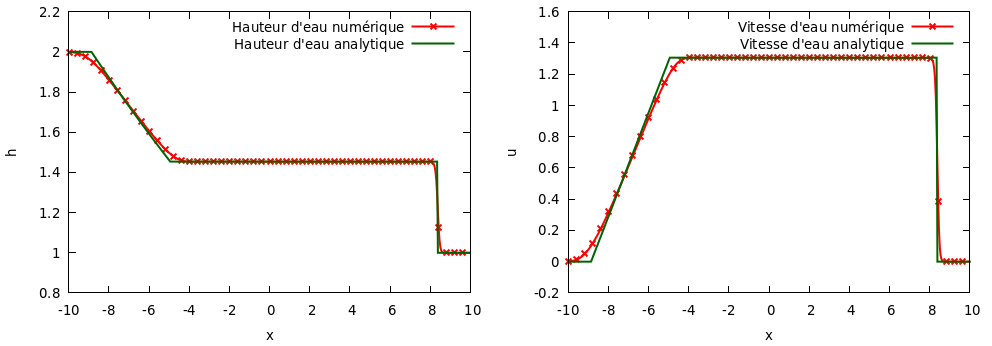
\includegraphics[width=\textwidth]{Piscineinfinie1.png}
		\caption{$t_{final}=2$}
	\end{subfigure}
	\begin{subfigure}[b]{0.9\textwidth}
		\centering
		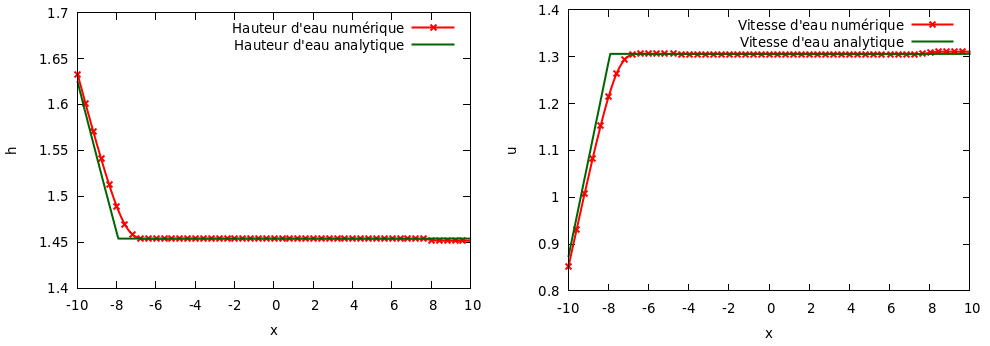
\includegraphics[width=\textwidth]{Piscineinfinie2.png}
		\caption{$t_{final}=3.2$}
		\label{fig:InfiniB}
	\end{subfigure}
	\begin{subfigure}[b]{0.9\textwidth}
		\centering
		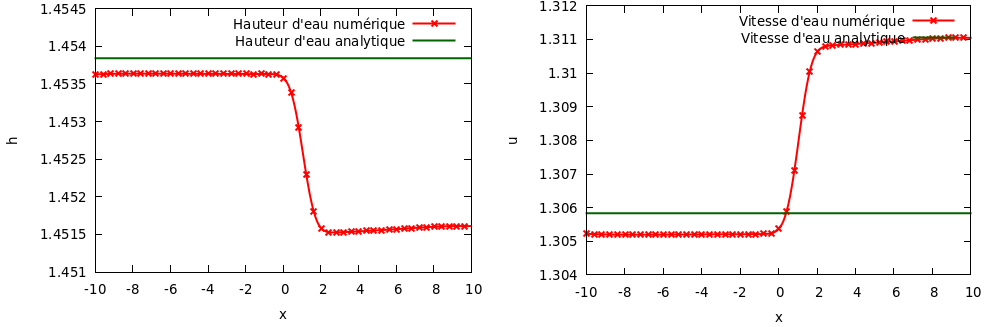
\includegraphics[width=\textwidth]{Piscineinfinie3.png}
		\caption{$t_{final}=6$}
		\label{fig:InfiniC}
	\end{subfigure}
	\caption{Illustration du cas avec un bassin infini sur un nombre de mailles $N=500$. Le coefficient $CFL$ vaut $0.5$. La figure (a) montre le système juste avant d'atteindre les bords, (b) juste après l'arrivée sur les bords, et (c) bien après.}
	\label{fig:Infini}
\end{figure}

La \cref{fig:Infini} illustre le bassin infini. Comparé aux cas du bassin fermé (\cref{sub@fig:Piscine1C,sub@fig:Piscine2C,sub@fig:Piscine3C}), la \cref{fig:InfiniC} ne montre aucun rebond sur les bords (et les deux solutions restent alignées\footnote{Il faut observer l'échelle de grandeur sur l'axe $y$ qui est différent d'une figure à l'autre.}). Pour un temps suffisamment grand, la surface d'eau semble complètement stable ($h\approx 1.45$, et $u\approx 1.30$), sauf en $x=0$ qui comporte la discontinuité initiale \footnote{En effet, $h_R=2,h_L=1$ autour de $x=0$.} dans le solveur de Riemann exact utilisé par la méthode de Godunov.


\subsection*{Question 5.}
\begin{problem}
Description, programmation et vérification du schéma de Rusanov. 
\end{problem}

\subsection*{Réponse} 

Le flux de Rusanov vectoriel est donné par 
\begin{align*}
	f(w_L,w_R) = \frac{f(w_L)+f(w_R)}{2} - \frac{\lambda}{2}(w_R-w_L)
\end{align*}
avec $$ \lambda = \max(\rho(A(w_L)),\, \rho(A(w_R))) $$
où $A$ désigne la matrice jacobienne de $f$. Dans le modèle de St-Venant, le rayon spectral vaut $\rho(A) = \vert u \vert + \sqrt{gh}$. On peut donc expliciter l'expression de $\lambda$ qui donne
$$
\lambda = \max(\vert u_L \vert + \sqrt{gh_L},\, \vert u_R \vert + \sqrt{gh_R})
$$
La programmation du schéma donne le code suivant. Les résultats obtenus sont présentés juste après.

\begin{lstlisting}[language=C, caption={Programmation du flux numérique de Rusanov.},breaklines]
void flux_rusanov(double *wL, double *wR, double *flux){
	double hL = wL[0];
	double uL = wL[1] / wL[0];
	double hR = wR[0];
	double uR = wR[1] / wR[0];
	double lambdaL = fabs(uL) + sqrt(_G*hL);
	double lambdaR = fabs(uR) + sqrt(_G*hR);
	double lambda = lambdaL>lambdaR ? lambdaL : lambdaR;
	double fL[2]; 
	double fR[2]; 
	fluxphy(wL, fL);
	fluxphy(wR, fR);
	flux[0] = (fL[0]+fR[0])/2. - lambda*(wR[0]-wL[0])/2.;
	flux[1] = (fL[1]+fR[1])/2. - lambda*(wR[1]-wL[1])/2.;
}	
\end{lstlisting}

\begin{figure}[H]
	\centering
	\begin{subfigure}[b]{0.9\textwidth}
		\centering
		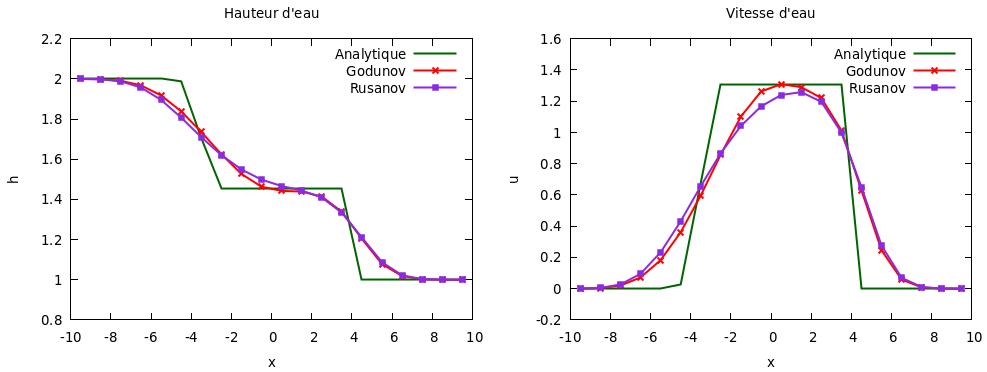
\includegraphics[width=\textwidth]{rusaVSgodu20.png}
		\caption{$N=20$}
	\end{subfigure}
	\begin{subfigure}[b]{0.9\textwidth}
		\centering
		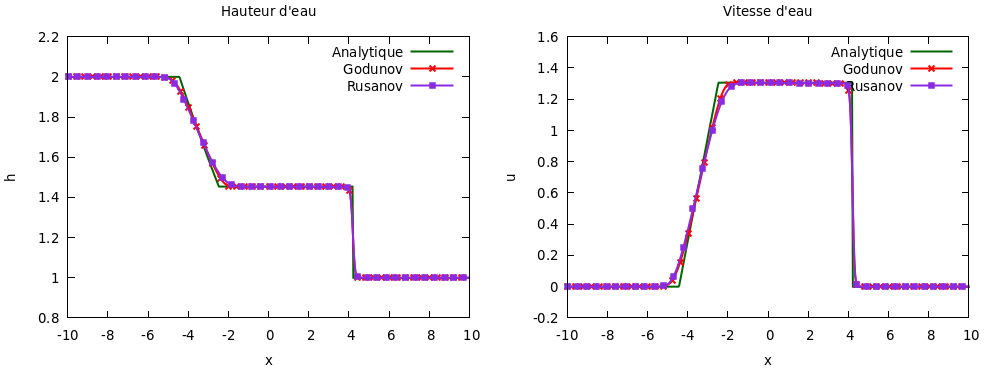
\includegraphics[width=\textwidth]{rusaVSgodu500.png}
		\caption{$N=500$}
	\end{subfigure}
	\caption{Observation des résultats obtenus par la méthode de Rusanov, à $t=1$, avec un coefficient $CFL=0.5$.}
	\label{fig:rusaVSgoduPlots}
\end{figure}
\noindent Les observations de précision sur la \cref{fig:rusaVSgoduPlots} sont confirmées par le graphique ci-bas, qui présente en plus des erreurs en norme $L^1$, les temps d'exécution. 

\begin{figure}[H]
	\centering
	\begin{subfigure}[b]{0.45\textwidth}
		\centering
		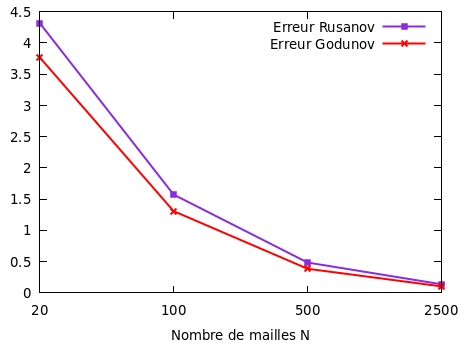
\includegraphics[width=\textwidth]{rusaVSgoduERR.png}
		\caption{Comparaison des erreurs}
		\label{fig:rusaVSgoduA}
	\end{subfigure}
	\begin{subfigure}[b]{0.45\textwidth}
		\centering
		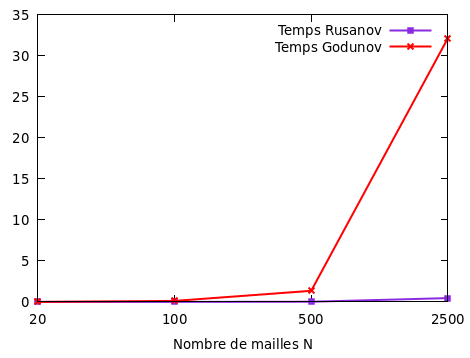
\includegraphics[width=\textwidth]{rusaVSgoduTIME.png}
		\caption{Comparaison des temps d'exécution}
		\label{fig:rusaVSgoduB}
	\end{subfigure}
	\caption{Comparaison du schéma de Rusanov et celui de Godunov. Les erreurs en (a) sont en norme $L^1$, et traduisent la somme des erreurs sur la hauteur d'eau, et sur la vitesse d'eau.}
	\label{fig:rusaVSgodu}
\end{figure}
Ces résultats confirment bien que le schéma de Rusanov est considérablement plus rapide (\cref{fig:rusaVSgoduB}), mais cela au coût de la précision (\cref{fig:rusaVSgoduA}). Dans les questions qui suivent, nous effectuerons des comparaisons encore plus détaillées entre le schéma de Godunov et un schéma utilisant le flux de Rusanov baptisé "VFRoe corrigé".



\subsection*{Question 6.}
\begin{problem}
Description du schéma VFRoe et calcul du flux numérique. 
\end{problem}

\subsection*{Réponse} 
Tout comme le flux de Godunov, le flux VFRoe repose sur le calcul de la solution du problème de Riemann au point $\sfrac{x}{t}=0$. Ce schéma se distingue par deux points principaux:
\begin{itemize}
	\item On remplace le solveur de Riemann $R(w_L, w_R, 0)$ exact par un solveur de Riemann approché $\tilde{R}(w_L, w_R, 0)$, qui est plus simple et plus rapide à calculer.
	\item On linéarise les équations régissant le problème autour d'un état moyen noté $\bar{y} = \dfrac{y_L+y_R}{2}$ (on retourne en variables primitives $y=(h,u)^T$ pour définir cet état moyen).
\end{itemize}
En récapitulatif, il faut résoudre, sur chaque volume fini du maillage, un problème de Riemann donné par:

\begin{align}
	\begin{cases}
		y_t + B(\bar{y})y_x = 0 \\
		y(x,0) = \begin{cases}
			y_L \hquad \text{si  } x < 0\\
			y_R \hquad \text{si  } x > 0 
		\end{cases}
	\end{cases}
\end{align}
En s'inspirant de l'équation de transport qui nous donne une solution au point $\sfrac{x}{t}=0$, nous pouvons écrire:
$$
y(0,t)=\frac{y_L+y_R}{2} - \frac{\text{sgn}(B(\bar{y}))}{2}(y_R-y_L)
$$
Le signe de la matrice $B(\bar{y})=\mymat{\bar u}{\bar h}{g}{\bar u}$ est lié à celui de ses valeurs propres ordonnées $\lambda_1$ et $\lambda_2$. 
\begin{itemize}
	\item Si $\lambda_1 < 0$ et $\lambda_2 < 0$, alors $\text{sgn}(B(\bar{y}))= -I_2$. On en déduit $y(0,t)=y_L$
	\item Si $\lambda_1 > 0$ et $\lambda_2 > 0$, alors $\text{sgn}(B(\bar{y}))= I_2$. On en déduit $y(0,t)=y_R$
	\item Si $\lambda_1 < 0$ et $\lambda_2 > 0$, alors le signe est donné par un polynôme du premier degré qui vaut $-1$ en $\lambda_1$, et $1$ en $\lambda_2$. On montre que ce polynôme vaut $Q(\lambda)= \dfrac{\lambda - \bar{u}}{\sqrt{g\bar h}}$. On obtient donc 
	$$
	\text{sgn}(B(\bar{y})) =Q(B(\bar{y}))= \frac{1}{\sqrt{g\bar{h}}}\mymat{0}{\bar{h}}{g}{0}
	$$
	On en déduit
	$$
	y(0,t)=\myvec{\frac{h_L+h_R}{2} - \frac{\bar{h}}{2\sqrt{g\bar{h}}}(u_R-u_L)}{\frac{u_L+u_R}{2} - \frac{g}{2\sqrt{g\bar{h}}}(h_R-h_L)}
	$$
\end{itemize}
Ce calcul fait, il faut retourner aux variables conservatives afin de définir la solution du problème de Riemann:
$$
\tilde{R}(w_L, w_R, 0) = \myvec{h(0,t)}{h(0,t)u(0,t)} = \myvec{w_1(0,t)}{w_2(0,t)} 
$$
Le flux numérique de VFRoe en découle par la relation 
$$
f_{VFRoe}(w_L, w_R) = f(\tilde{R}(w_L, w_R, 0))
$$
$f$ étant défini en variables conservatives par $ f(w) = \myvec{w_2}{\frac{w_2^2}{w_1} + \frac{gw_1^2}{2}}$.

\subsection*{Question 7.}
\begin{problem}
Programmation du schéma de VFRoe.
\end{problem}

\subsection*{Réponse} 

Les indications de la question précédente sont implémentées dans la fonction $\verb|riem_vfroe|$ précisée ci-bas.

\begin{lstlisting}[language=C, caption={Programmation du flux numérique VFRoe.},breaklines]
void riem_vfroe(double *wL, double *wR, double z, double *w){
    double hL = wL[0];
    double uL = wL[1] / wL[0];
    double hR = wR[0];
    double uR = wR[1] / wR[0];
    double hBar = (hL + hR) /2.0;
    double uBar = (uL + uR) /2.0;
    double cBar = sqrt(_G * hBar);
    double lambda_1 = uBar - cBar;
    double lambda_2 = uBar + cBar;

	// Calcul de y(0,t) par distinction de cas
    double h, u;
    if ((lambda_1 > 0) && (lambda_2 > 0)){
        h = hL;
        u = uL;
    } else if (lambda_1 < 0 && lambda_2 < 0){
        h = hR;
        u = uR;
    // Cas lambda_1 < 0 && lambda_2 > 0
    } else {
        h = hBar - (hBar*(uR-uL))/(2*sqrt(_G*hBar));
        u = uBar - (_G*(hR-hL))/(2*sqrt(_G*hBar));
    }

    w[0] = h;
    w[1] = h*u;
}	
\end{lstlisting}
Les résultats sont présentés à la \cref{fig:VFRoeNormal}. On observe effectivement les mêmes résultats que ceux obtenus par les schémas de Godunov (questions 2, 3, et 4) et Rusanov (question 5).

\begin{figure}[H]
	\centering
	\begin{subfigure}[b]{0.8\textwidth}
		\centering
		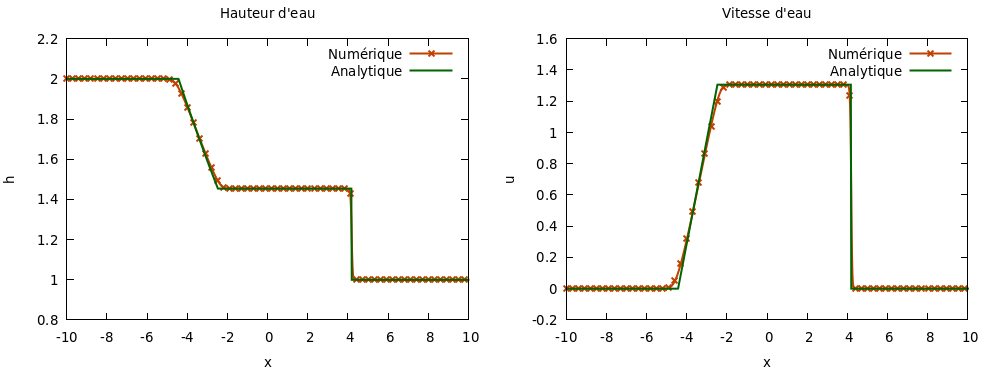
\includegraphics[width=\textwidth]{VFRoeNormal.png}
		\caption{$t_{final}=1$}
	\end{subfigure}
	\begin{subfigure}[b]{0.8\textwidth}
		\centering
		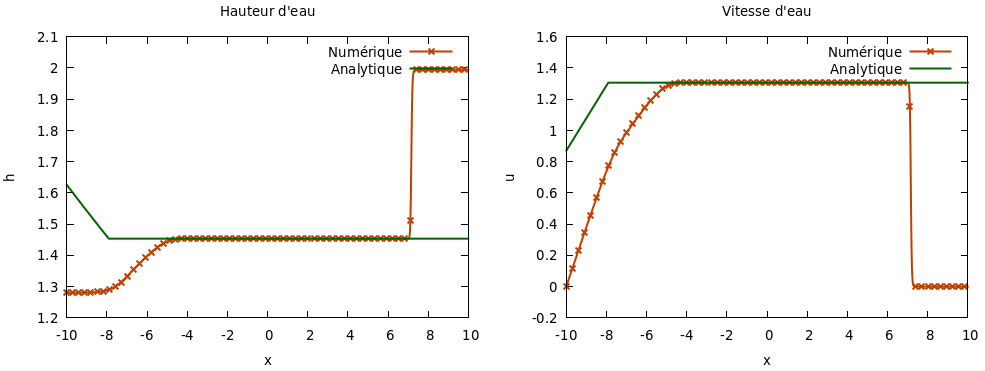
\includegraphics[width=\textwidth]{VFRoeBorne.png}
		\caption{$t_{final}=3.2$ sur dans le bassin fermé}
	\end{subfigure}
	\begin{subfigure}[b]{0.8\textwidth}
		\centering
		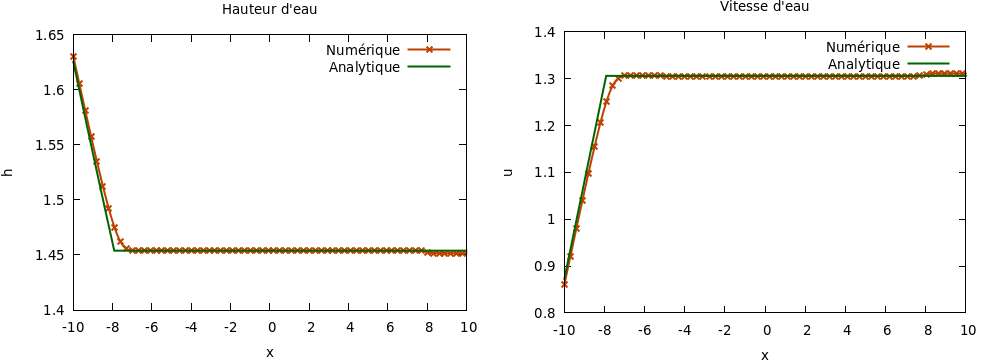
\includegraphics[width=\textwidth]{VFRoeInfinie.png}
		\caption{$t_{final}=3.2$ sur dans le bassin infinie}
	\end{subfigure}
	\caption{Illustration des résultats obtenus par le schéma VFRoe pour un nombre de mailles $N=1000$. Le coefficient $CFL$ vaut $0.5$. La figure (a) montre le système avant d'atteindre les bords du domaine sur lesquels on applique des conditions particulières en fonction qu'on soit sur un bassin fermé ou un bassin infini, (b) après l'arrivée des ondes dans un bassin fermé, et (c) après l'arrivée des ondes dans un bassin infini.}
	\label{fig:VFRoeNormal}
\end{figure}


\begin{problem}
Vérifions que le schéma VFRoe ne donne pas toujours la bonne solution (en choisissant un problème de Riemann associé à une onde de détente qui traverse une valeur propre nulle).
\end{problem}

\subsection*{Réponse} 

On vérifie que le problème de Riemann dont l'état initial est défini par
\begin{align*}
	y(x,0) = \begin{cases}
		\myvec{h_L=1}{u_L=-1} \hquad &\text{si  } x < 0\\
		\myvec{h_R=0.25}{u_R=u_L + 2\sqrt{g}(\sqrt{h_L}-\sqrt{h_R})} \hquad &\text{si  } x > 0 
	\end{cases}
\end{align*}
traverse bien une valeur propre $\lambda_1 = u-\sqrt{gh}$ nulle car $u_L-\sqrt{gh_L} < 0$ et $u_R-\sqrt{gh_R} > 0$. Dorénavant, cet état sera l'état initial pour nos simulations.

\begin{figure}[H]
	\centering
	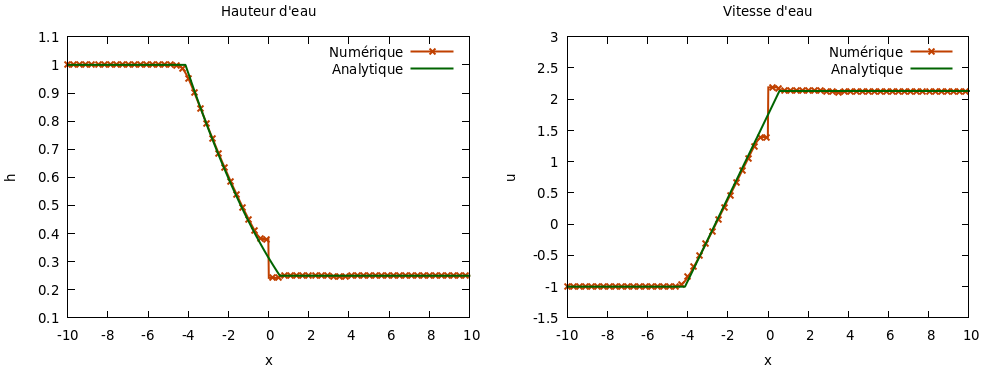
\includegraphics[width=\textwidth]{VFRoePointSonique.png}
	\caption{Mauvaise solution obtenue par le schéma VFRoe lorsque le schéma traverse une valeur propre nulle. On constate effectivement que la solution numérique proche du point de discontinuité $x=0$ ne correspond pas à la solution analytique exacte. Le nombre de mailles ici vaut $N=1000$. Le coefficient $CFL$ vaut $0.5$.}
	\label{fig:VFRoePasNormal}
\end{figure}
\noindent Comparé au schéma de Godunov (cf. \cref{fig:SolGodunov500}) qui donnait des résultats correctes (même aux points de discontinuité), la non-concordance des solutions ici peut-être dû au fait que le flux de VFRoe ne vérifie pas le critère d'entropie (géométrique) de Lax, alors que le flux de Godunov le fait bien.  

\subsection*{Question 8.}
\begin{problem}
Correction entropique qui utilise le flux de Rusanov aux points "soniques" (c'est-à-dire les points où la vitesse du "son" $c = \sqrt{gh}$ est égale à $ \pm  u$).
\end{problem}

\subsection*{Réponse} 

Pour appliquer cette correction, il suffit, avant d'appliquer le flux VFRoe, de vérifier que les vitesses de chacune des ondes ($\lambda_1 = u - c$ et $\lambda_2 = u + c$) aux interfaces d'une maille ne sont pas de signes opposés ($\lambda_{1L} < 0$ et $\lambda_{1R} > 0$ ou $\lambda_{2L} < 0$ et $\lambda_{2R} > 0$). Si cette condition est vérifiée, on applique le flux de Rusanov à la place. Tout ceci correspond à une modification de la fonction de calcul du flux numérique comme suit:

\begin{lstlisting}[language=C, caption={Application d'une correction entropique qui utilise le flux de Rusanov aux points "soniques".},breaklines]
void fluxnum(double* a, double* b, double* flux) {
	double w[2];       
	double *wL = a;
	double *wR = b;    
	double hL = wL[0];
	double uL = wL[1] / wL[0];
	double hR = wR[0];
	double uR = wR[1] / wR[0];	
	double lambda_1L = uL - sqrt(_G*hL);
	double lambda_2L = uL + sqrt(_G*hL);
	double lambda_1R = uR - sqrt(_G*hR);
	double lambda_2R = uR + sqrt(_G*hR);
	// Correction du flux
    if ((lambda_1L<0 && lambda_1R>0) || (lambda_2L<0 && lambda_2R>0))
        flux_rusanov(a, b, flux);
    else{
        riem_vfroe(a, b, 0., w);
        fluxphy(w, flux);
    }
    fluxphy(w, flux);
}	
\end{lstlisting}
On obtient le résultat ci-dessous.
\begin{figure}[H]
	\centering
	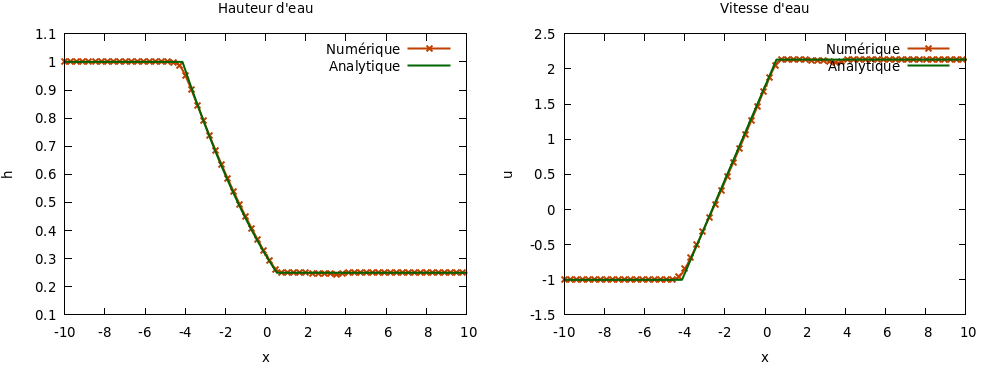
\includegraphics[width=\textwidth]{VFRoeRusanov.png}
	\caption{Correction du schéma VFRoe par un schéma de Rusanov aux points soniques. Comparé à la \cref{fig:VFRoePasNormal}, on constate effectivement que la discontinuité au point $x=0$ disparait. Le nombre de mailles vaut $N=1000$. Le coefficient $CFL$ vaut $0.5$.}
	\label{fig:VFRoeRusanov}
\end{figure}



\subsection*{Question 9.}
\begin{problem}
Comparaison du schéma de VFRoe corrigé par le flux de Rusanov avec le schéma de Godunov en termes de précision et de temps de calcul.
\end{problem}

\subsection*{Réponse} 

Les résultats sont présentés ci-bas, aux \cref{fig:VFRoeVSgoduPlots,fig:VFRoeVSgodu}, où la notation "VFRoe corrigé" indique le schéma de VFRoe corrigé par le flux de Rusanov aux points "soniques".

\begin{figure}[H]
	\centering
	\begin{subfigure}[b]{0.8\textwidth}
		\centering
		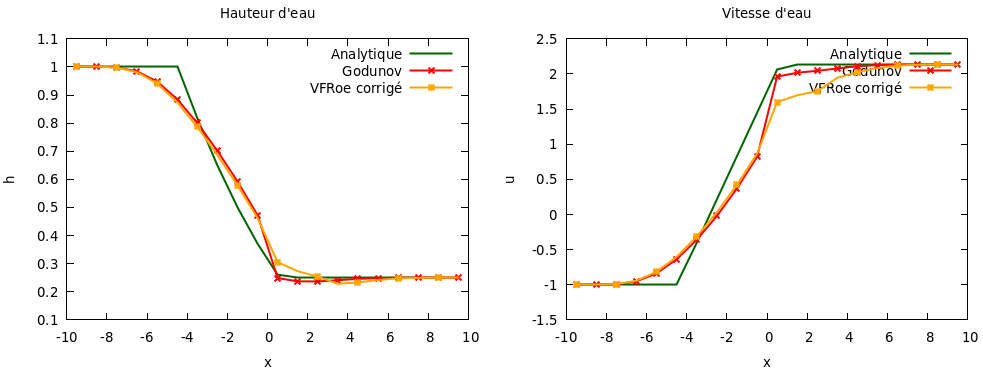
\includegraphics[width=\textwidth]{VFRoeVSGodu1.png}
		\caption{$N=20$}
		\label{fig:VFRoeVSgoduPlotsA}
	\end{subfigure}
	\begin{subfigure}[b]{0.8\textwidth}
		\centering
		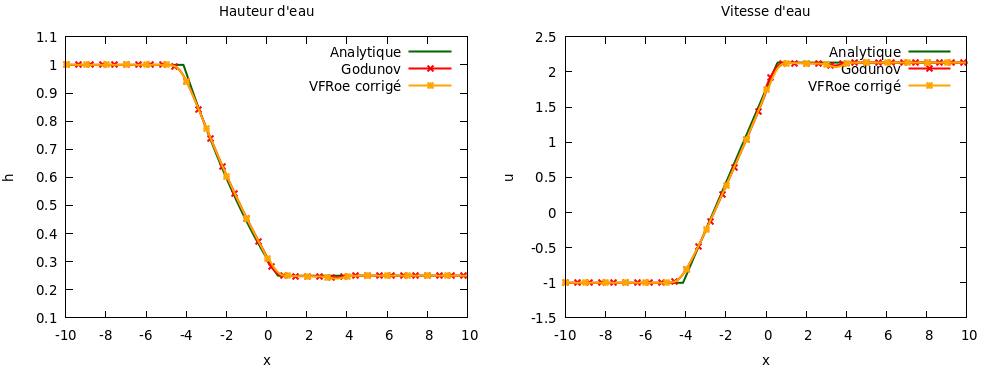
\includegraphics[width=\textwidth]{VFRoeVSGodu2.png}
		\caption{$N=500$}
	\end{subfigure}
	\caption{Observation des résultats obtenus par le schéma VFRoe corrigé (en jaune), à $t=1$, avec un coefficient $CFL=0.5$.}
	\label{fig:VFRoeVSgoduPlots}
\end{figure}

\noindent Pour $N$ très faible, le schéma de Godunov semble être le meilleur en termes de précision (\cref{fig:VFRoeVSgoduPlotsA}), mais dès que le nombre de mailles augmente, il n'y a plus d'avantages à utiliser cette technique. En fait, la \cref{fig:VFRoeVSgodu} (ainsi que les \cref{tab:errL1,tab:time}) montre que le schéma VFRoe corrigé est considérablement plus rapide que le schéma de Godunov, tout en gardant une précision élevée; il serait donc judicieux d'utiliser le schéma VFRoe corrigé pour des simulations raffinées.

\begin{table}[h!]
    \centering
    \begin{tabular}{l c c}
		\multicolumn{3}{c}{\tabhead{Erreurs}} \\
        \toprule
        \tabhead{N} & \tabhead{VFRoe corrigé} & \tabhead{Godunov} \\
        \midrule
        \tabhead{$20$} & 4.115179 & 2.839234 \\
        \tabhead{$100$} & 1.316861 & 1.081817 \\
        \tabhead{$500$} & 0.391413 & 0.355618 \\
        \tabhead{$2500$} & 0.106957 & 0.103105 \\
        \bottomrule
    \end{tabular}
	\caption{Comparaison du schéma VFRoe corrigé et celui de Godunov pour les erreurs en norme $L^1$, traduisent la somme des erreurs sur la hauteur et la vitesse d'eau. L'illustration est fournie à la \cref{fig:VFRoeVSgoduA}.}
	\label{tab:errL1}
\end{table}

\begin{table}[h!]
    \centering
    \begin{tabular}{l c c}
		\multicolumn{3}{c}{\tabhead{Temps d'execution}} \\
		\toprule
        \tabhead{N} & \tabhead{VFRoe corrigé} & \tabhead{Godunov} \\
        \midrule
        \tabhead{$20$} & 0.118 & 0.169 \\
        \tabhead{$100$} & 0.182 & 0.178 \\
        \tabhead{$500$} & 0.203 & 1.060 \\
        \tabhead{$2500$} & 0.700 & 22.144 \\
        \bottomrule
    \end{tabular}
	\caption{Comparaison du schéma VFRoe corrigé et celui de Godunov pour les temps exécution (en seconde), sans tenir compte du temps système. L'illustration est fournie à la \cref{fig:VFRoeVSgoduB}.}
	\label{tab:time}
\end{table}


\begin{figure}[H]
	\centering
	\begin{subfigure}[b]{0.4\textwidth}
		\centering
		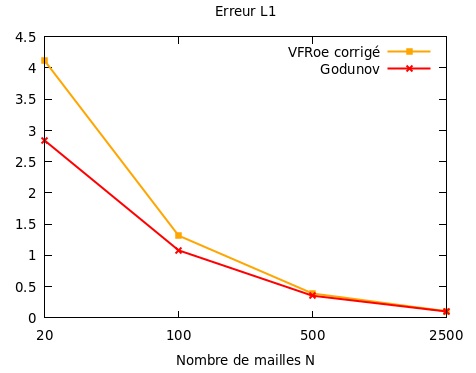
\includegraphics[width=\textwidth]{VFRoeVSgoduERR.png}
		\caption{Comparaison des erreurs}
		\label{fig:VFRoeVSgoduA}
	\end{subfigure}
	\begin{subfigure}[b]{0.4\textwidth}
		\centering
		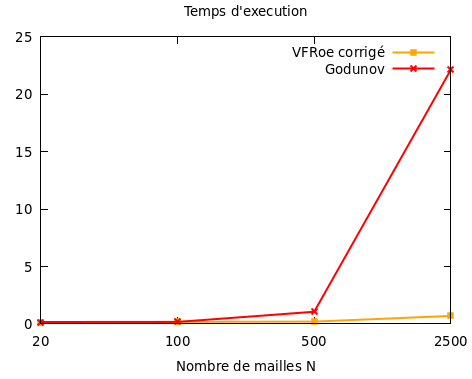
\includegraphics[width=\textwidth]{VFRoeVSgoduTIME.png}
		\caption{Comparaison des temps d'exécution}
		\label{fig:VFRoeVSgoduB}
	\end{subfigure}
	\caption{Comparaison du schéma de VFRoe corrigé et celui de Godunov. Les figures (a) et (b) correspondent aux \cref{tab:errL1,tab:time} respectivement.}
	\label{fig:VFRoeVSgodu}
\end{figure}



\begin{figure}[H]
	\centering
	\begin{subfigure}[b]{0.4\textwidth}
		\centering
		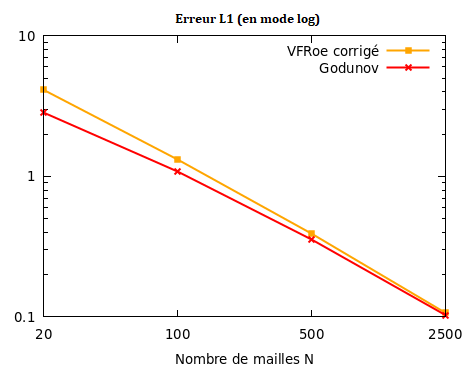
\includegraphics[width=\textwidth]{VFRoeVSgoduERRLOG.png}
		\caption{Comparaison des erreurs}
	\end{subfigure}
	\begin{subfigure}[b]{0.4\textwidth}
		\centering
		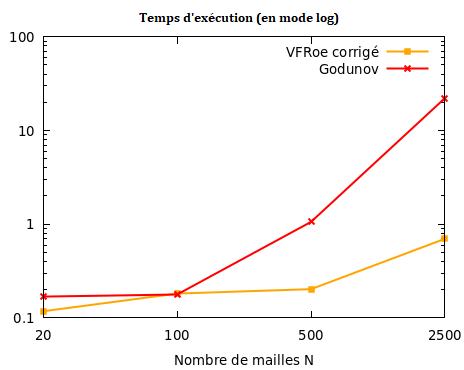
\includegraphics[width=\textwidth]{VFRoeVSgoduTIMELOG.png}
		\caption{Comparaison des temps d'exécution}
	\end{subfigure}
	\caption{Comparaison du schéma de VFRoe corrigé et celui de Godunov en échelle "log". Ces données correspondent aux \cref{tab:errL1,tab:time} respectivement, déjà illustrés aux figures \cref{fig:VFRoeVSgoduA,fig:VFRoeVSgoduB}. Ces résultats confirment bien que le schéma VFRoe corrigé est à préconiser pour des simulations fines, vu qu'il est précis et rapide.}
	\label{fig:VFRoeVSgodu}
\end{figure}


\subsection*{Question 10.}
\begin{problem}
	Calcul du flux de Roe\footnote{Dans cette question, nous utilisons le flux VFRoe, et non le flux de Roe comme demandé.}. Programmation et test du schéma de Roe. Vérification qu'il a besoin lui aussi d'une correction entropique. Test du schéma de Roe avec correction entropique.
\end{problem}

\subsection*{Réponse} 

La correction entropique en question, appliquée aux cas $\lambda_{1L} < 0, \lambda_{1R} > 0$, et $\lambda_{2L} < 0, \lambda_{2R} > 0$, consiste à rajouter une viscosité artificielle aux flux 
$$
\tilde{f}(w_L,w_R) = f(w_L,w_R) + \frac{\varepsilon}{2} (w_R-w_L)
$$
$\varepsilon$ étant choisi de façon à minimiser le décalage de chacune des valeurs propres $\lambda_1$ et $\lambda_2$ de la valeur $0$. Vu que le même flux est appliqué aux deux ondes, on obtient 
$$
\varepsilon = \max{(\min{(-\lambda_{1L}, \lambda_{1R})}, \min{(-\lambda_{2L}, \lambda_{2R})})}.
$$ 
L'implémentation de cette correction s'effectue indépendamment du calcul de flux VFRoe. On rajoute la viscosité artificielle $\varepsilon$ comme l'indique le code de calcul suivant.


\begin{lstlisting}[language=C, caption={Application d'une correction entropique "facile" aux flux VFRoe afin de traiter les points soniques.},breaklines]
void fluxnum(double* a, double* b, double* flux) {
	double w[2];       
	double *wL = a;
	double *wR = b;    
	double hL = wL[0];
	double uL = wL[1] / wL[0];
	double hR = wR[0];
	double uR = wR[1] / wR[0];	
	double lambda_1L = uL - sqrt(_G*hL);
	double lambda_2L = uL + sqrt(_G*hL);
	double lambda_1R = uR - sqrt(_G*hR);
	double lambda_2R = uR + sqrt(_G*hR);
	double epsL = 0;
	double epsR = 0;
	// Calcul de la viscosité
	if (lambda_1L < 0 && lambda_1R > 0){
		epsL = fmin(-lambda_1L, lambda_1R);
	}
	if (lambda_2L < 0 && lambda_2R > 0)
		epsR = fmin(-lambda_2L, lambda_2R);
	double eps = fmax(epsL,epsR);
	// Flux VFRoe
	riem_vfroe(a, b, 0., w);
	fluxphy(w, flux);
	// Correction du flux VFRoe par rajout de la viscosité
	for (int i = 0; i < 2; i++)
	{
		flux[i] -= eps/2.0  * (wR[i]-wL[i]);
	}
}	
\end{lstlisting}
On obtient effectivement une correction du résultat, comme le montre la figure ci-bas:

\begin{figure}[H]
	\centering
	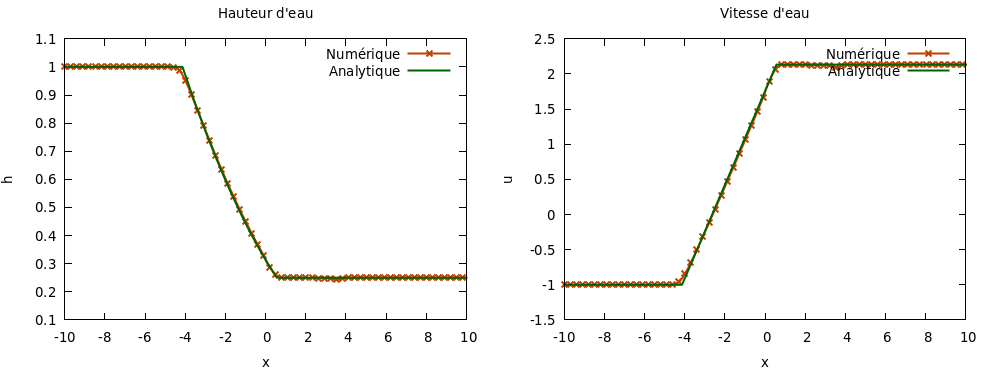
\includegraphics[width=\textwidth]{VFRoeCorrrectionEntropique.png}
	\caption{Correction entropique "facile" du schéma VFRoe. Comparé à la \cref{fig:VFRoePasNormal}, on constate effectivement que la discontinuité au point $x=0$ disparait. Le nombre de mailles ici vaut $N=1000$. Le coefficient $CFL$ vaut $0.5$.}
	\label{fig:VFRoeEntropique}
\end{figure}




\subsection*{Question 11.}
\begin{problem}
	Programmation de la méthode MUSCL pour le schéma VFRoe sans correction entropique avec intégration en temps de RK2.
\end{problem}

\subsection*{Réponse} 

La méthode MUSCL consiste à calculer des pentes en espace et en temps que l'on applique aux centres des mailles\footnote{Le lecteur est renvoyé à la question 4 de la partie 2 du T.P. \#1, ou à la question 8 du T.P. \#3 pour une description détaillée de la méthode MUSCL}. Ici, on ne s'intéresse qu'à la correction MUSCL en espace, et les itérations en temps seront gérés par un schéma de Runge-Kutta d'ordre 2 que nous détaillons ci-bas. Après l'application des pentes MUSCL en espace, on obtient les valeurs $w_{+_L},w_{+_R},w_{-_L}$, et $w_{-_R}$; on fait l'approximation $w_i(t) \approx w(x_i,t)$ pour se retrouver avec:
\begin{align*}
	w'_i(t) + \frac{f(w_{+_{L}}(t),w_{+_{R}}(t)) - f(w_{-_L}(t),w_{-_R}(t))}{\Delta x} = 0
\end{align*}
qu'on résout par une intégration en temps RK2. En d'autres termes, on calcule $k_1$ et $k_2$ tel que 
\begin{align*}
	k_1 &= \frac{\Delta t}{\Delta x} \left[ f(w_{+_{L}},w_{+_{R}} - f(w_{-_L},w_{-_R}) \right]\\
	k_2 &= \frac{\Delta t}{\Delta x} \left[  f(w_{+_{L}}+k_1,w_{+_{R}}+k_1) - f(w_{-_L}+k_1,w_{-_R}+k_1) \right]
\end{align*}
enfin, on pose
$$
w^{n+1}_i = w^{n}_i + \frac{1}{2}(k_1 + k_2)
$$

\noindent Les modifications à apporter au code pour implémenter la méthode MUSCL se situent toutes au niveau de la fonction principale de résolution $\verb|godunov_solve|$. On y retrouve le calcul des pentes en espace, celui des pentes en temps, et leur application au schéma numérique.

\begin{lstlisting}[language=C, caption={Application de la correction MUSCL en espace, et d'un schéma de Runge-Kutta d'ordre 2 en temps. La fonction "fluxnum" observée correspond au flux VFRoe sans correction entropique.},breaklines]
void godunov_solve(godunov* gd, double tmax) {
    double tnow = 0;
    int m = gd->m;
    while (tnow < tmax) {
        double vmax = 0;
        // Calcul de la vitesse max
        for (int i = 0; i < gd->N + 2; i++) {
            double vloc = lambda_max(gd->un + m * i);
            vmax = vmax > vloc ? vmax : vloc;
        }
        // Calcul des pentes pour MUSCL en espace
        double si[m*(gd->N+2)], ri[m*(gd->N+2)];
        for (int i = 1; i < gd->N + 1; i++) {
            for (int iv = 0; iv < m; iv++) {
                double alpha = (gd->un[i * m + iv] - gd->un[(i-1) * m + iv])/gd->dx;
                double beta = (gd->un[(i+1) * m + iv] - gd->un[i * m + iv])/gd->dx;
                double gamma = (gd->un[(i+1) * m + iv] - gd->un[(i-1) * m + iv])/(2.0*gd->dx);
                si[i * m + iv] = minmod(alpha, beta, gamma);
            }   
        }
		// Calcul du pas de temps
        gd->dt = gd->cfl * gd->dx / vmax;
		// Application du schéma de Runge Kutta d'ordre 2 en temps
        for (int i = 1; i < gd->N + 1; i++) {            
            double uLplus[2], uRplus[2], uLmoins[2], uRmoins[2];
            for (int iv = 0; iv < m; iv++) {
                uLplus[iv] = gd->un[i*m+iv] + si[i*m+iv]*gd->dx/2.0;
                uRplus[iv] = gd->un[(i+1)*m+iv] - si[(i+1)*m+iv]*gd->dx/2.0;
                uLmoins[iv] = gd->un[(i-1)*m+iv] + si[(i-1)*m+iv]*gd->dx/2.0;
                uRmoins[iv] = gd->un[i*m+iv] - si[i*m+iv]*gd->dx/2.0;
            }
            double fluxPlus[m];
            double fluxMoins[m];
            fluxnum(uLplus, uRplus, fluxPlus);
			fluxnum(uLmoins, uRmoins, fluxMoins);
			// Pente RungeKutta k1
            double k1[m]; 
            for (int iv = 0; iv < m; iv++) {
                k1[iv] = - gd->dt * (fluxPlus[iv] - fluxMoins[iv])/gd->dx;
            }

            double uLplusPrime[m], uRplusPrime[m], uLmoinsPrime[m], uRmoinsPrime[m];
            for (int iv = 0; iv < m; iv++) {
                uLplusPrime[iv] = uLplus[iv] + k1[iv];
                uRplusPrime[iv] = uRplus[iv] + k1[iv];

                uLmoinsPrime[iv] = uLmoins[iv] + k1[iv];
                uRmoinsPrime[iv] = uRmoins[iv] + k1[iv];
            }
            double fluxPlusPrime[m];
            double fluxMoinsPrime[m];
            fluxnum(uLplusPrime, uRplusPrime, fluxPlusPrime);
            fluxnum(uLmoinsPrime, uRmoinsPrime, fluxMoinsPrime);
			// Pente RungeKutta k2
            double k2[m]; 
            for (int iv = 0; iv < m; iv++) {
                k2[iv] = - gd->dt * (fluxPlusPrime[iv] - fluxMoinsPrime[iv])/gd->dx;
            }
            for (int iv = 0; iv < m; iv++) {
                gd->unp1[i * m + iv] =  gd->un[i*m+iv] + (k1[iv] + k2[iv]) / 2.0;
            }
        }
        // Mise à jour du temps
        tnow += gd->dt;
		// Conditions aux limites
        int i = 0;
        solexacte(gd->xi[i], tnow, gd->unp1 + i * m);
        i = gd->N + 1;
        solexacte(gd->xi[i], tnow, gd->unp1 + i * m);
		// Copie des valeurs
        memcpy(gd->un, gd->unp1, (gd->N + 2) * m * sizeof(double));
    }
    gd->tfin = tnow;
}
\end{lstlisting}
	
\noindent La programmation de la correction MUSCL en espace, et d'un schéma de Runge-Kutta d'ordre 2 en temps ne produit pas exactement les même résultats que ceux de VFRoe sur lesquels la correction entropique a été appliquée (cf. \cref{fig:VFRoeEntropique,fig:MusclNEW}). En comparant cette fois les \cref{fig:VFRoePasNormal,fig:MusclNEW}\footnote{On y observe le point sonique à traiter en $x=0$.}, on observe que la discontinuité au point $x=0$ à entièrement disparue, mais qu'une nouvelle discontinuité en $x=-4$ s'est formée. Vu que le problème du point sonique en $x=0$ a été résolu, on en déduit que la correction entropique n'est plus nécessaire.


\begin{figure}[H]
	\centering
	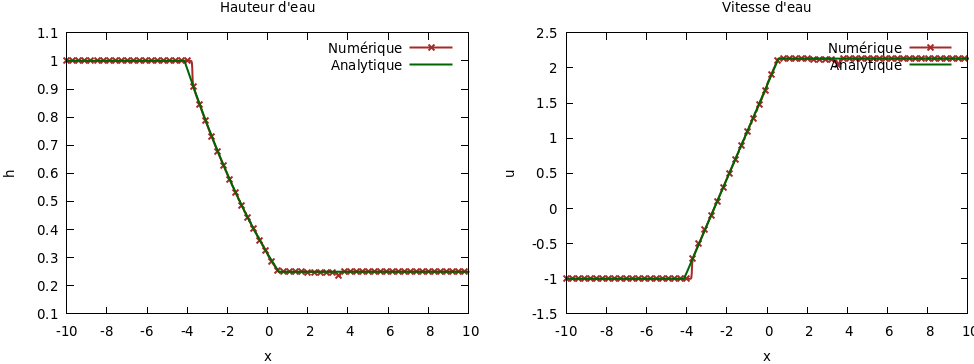
\includegraphics[width=\textwidth]{MusclNEW2.png}
	\caption{Observation des résultats obtenus par la correction MUSCL en espace et un schéma RK2 en temps, appliquée au schéma VFRoe. Les conditions initiales sont les même que celles utilisées jusqu'a présent, en plus d'avoir la garantie du point sonique i.e $h_L=1$, $u_L=-1$, $h_R=0.25$, $u_R = u_L + 2\sqrt{g}(\sqrt{h_L}-\sqrt{h_R})$.}
	\label{fig:MusclNEW}
\end{figure}


\noindent Afin d'améliorer les résultats\footnote{Il s'agit de supprimer la discontinuité en $x=-4$.}, on décide d'implémenter une correction MUSCL pour le schéma VFRoe en espace et en temps. La programmation de ce cette méthode (dont le code de calcul est fourni ci-bas) produit les mêmes résultats que ceux obtenus pour le schéma de Roe avec la correction entropique (\cref{fig:VFRoeEntropique,fig:Muscl2}). En comparant les \cref{fig:MusclNEW,fig:Muscl2}, on constate effectivement l'amélioration des résultats. Cette correction MUSCL (en temps et en espace) ne nécessite guère de correction entropique. Les méthodes de types MUSCL sont en fait les meilleures méthodes pour corriger les points soniques, car elles sont plus pratiques.


\begin{lstlisting}[language=C, caption={Application de la correction MUSCL. La fonction "fluxnum" observée correspond au flux VFRoe sans correction entropique.},breaklines]
void godunov_solve(godunov* gd, double tmax) {
	double tnow = 0;
	int m = gd->m;
	while (tnow < tmax) {
		double vmax = 0;
		// calcul de la vitesse max
		for (int i = 0; i < gd->N + 2; i++) {
			double vloc = lambda_max(gd->un + m * i);
			vmax = vmax > vloc ? vmax : vloc;
		}
		// Calcul des pentes pour MUSCL
		double si[m*(gd->N+2)], ri[m*(gd->N+2)];
		for (int i = 1; i < gd->N + 1; i++) {
			for (int iv = 0; iv < m; iv++) {
				double alpha = (gd->un[i * m + iv] - gd->un[(i-1) * m + iv])/gd->dx;
				double beta = (gd->un[(i+1) * m + iv] - gd->un[i * m + iv])/gd->dx;
				double gamma = (gd->un[(i+1) * m + iv] - gd->un[(i-1) * m + iv])/(2.0*gd->dx);
				si[i * m + iv] = minmod(alpha, beta, gamma);
			}   
			ri[i * m + 0] = -si[i * m +1];
			ri[i * m + 1] = -(_G*gd->un[i*m] - gd->un[i*m+1]*gd->un[i*m+1]/(gd->un[i*m]*gd->un[i*m]))*si[i*m+0] - 2*si[i*m+1]*gd->un[i*m+1]/gd->un[i*m];
		}
		// Pas de temps
		gd->dt = gd->cfl * gd->dx / vmax;
		// Application du flux numerique
		for (int i = 1; i < gd->N + 1; i++) {
			double flux[m];
			double uL[2], uR[2];
			// Application de MUSCL à droite
			for (int iv = 0; iv < m; iv++) {
				uL[iv] = gd->un[i*m+iv] + si[i*m+iv]*gd->dx/2.0 + ri[i*m+iv]*gd->dt/2.0;
				uR[iv] = gd->un[(i+1)*m+iv] - si[(i+1)*m+iv]*gd->dx/2.0 + ri[(i+1)*m+iv]*gd->dt/2.0;
			}
			fluxnum(uL, uR, flux);
			for (int iv = 0; iv < m; iv++) {
				gd->unp1[i * m + iv] =
					gd->un[i * m + iv] - gd->dt / gd->dx * flux[iv];
			}
			// Application de MUSCL à gauche
			for (int iv = 0; iv < m; iv++) {
				uL[iv] = gd->un[(i-1)*m+iv] + si[(i-1)*m+iv]*gd->dx/2.0 + ri[(i-1)*m+iv]*gd->dt/2.0;
				uR[iv] = gd->un[i*m+iv] - si[i*m+iv]*gd->dx/2.0 + ri[i*m+iv]*gd->dt/2.0;
			}
			fluxnum(uL, uR, flux);
			for (int iv = 0; iv < m; iv++) {
				gd->unp1[i * m + iv] += gd->dt / gd->dx * flux[iv];
			}
		}
		// Mise à jour
		tnow += gd->dt;
		// Conditions au bord
		int i = 0;
		solexacte(gd->xi[i], tnow, gd->unp1 + i * m);
		i = gd->N + 1;
		solexacte(gd->xi[i], tnow, gd->unp1 + i * m);
		// Preparation pour la prochaine etape
		memcpy(gd->un, gd->unp1, (gd->N + 2) * m * sizeof(double));
	}
	gd->tfin = tnow;
}	
\end{lstlisting}

\begin{figure}[H]
	\centering
	\begin{subfigure}[b]{0.8\textwidth}
		\centering
		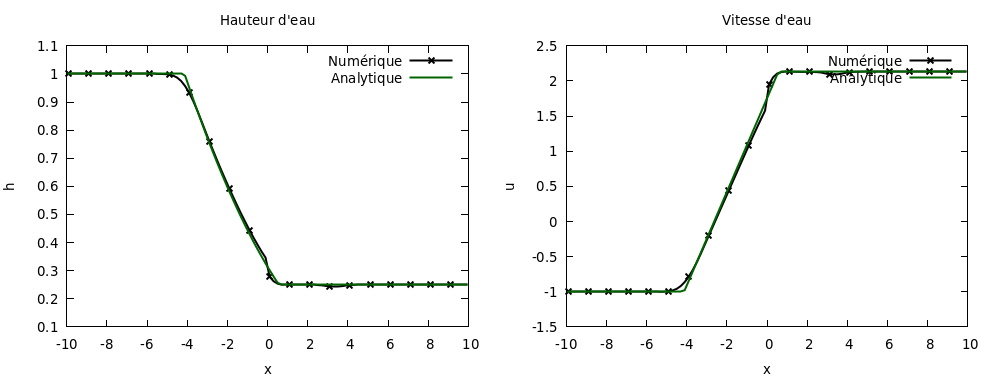
\includegraphics[width=\textwidth]{Muscl1.png}
		\caption{$N=100$}
	\end{subfigure}
	\begin{subfigure}[b]{0.8\textwidth}
		\centering
		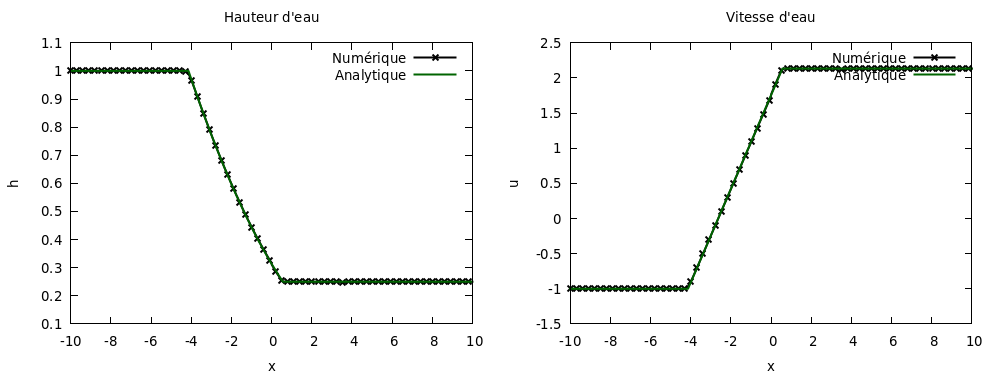
\includegraphics[width=\textwidth]{Muscl2.png}
		\caption{$N=1000$}
		\label{fig:Muscl2}
\end{subfigure}
	\caption{Observation des résultats obtenus par la correction MUSCL en espace et en temps appliquée au schéma VFRoe. Les conditions initiales sont les mêmes que celles utilisées jusqu'à présent, en plus d'avoir la garantie du point sonique i.e $h_L=1$, $u_L=-1$, $h_R=0.25$, $u_R = u_L + 2\sqrt{g}(\sqrt{h_L}-\sqrt{h_R})$.}
	\label{fig:Muscl}
\end{figure}


\end{document}
